\documentclass{article}
\usepackage[utf8]{inputenc}
\usepackage[italian]{babel}
\usepackage{amsmath}
\usepackage{amssymb}
\usepackage{siunitx}
\usepackage{tabularray}
\usepackage{graphicx}
\usepackage{float}
% \usepackage{minted}
\usepackage[bottom]{footmisc}
\usepackage[page]{appendix}
\usepackage[labelformat=simple, justification=centering]{subfig}
\renewcommand{\thesubfigure}{}
\newcommand*{\diam}{\varnothing}
\newcommand*{\best}[1]{{#1}_\text{best}}
\newcommand*{\bestp}[1]{{\left(#1\right)}_\text{best}}
\newcommand*{\pbest}[1]{\left({#1}_\text{best}\right)}
\newcommand*{\pbestp}[1]{\left({\left(#1\right)}_\text{best}\right)}
\newcommand*{\errrel}[1]{\frac{\delta #1}{{#1}_\text{best}}}
\title{
  Laboratorio di Fisica 1\\
  R12: Misura della velocità del suono
}
\author{Gruppo 15: Bergamaschi Riccardo, Graiani Elia, Moglia Simone}
\date{28/05/2024 – 04/06/2024}
\makeindex
\begin{document}

\maketitle

\begin{abstract}
  Il gruppo di lavoro ha misurato la velocità del suono mediante
  un apparato sperimentale detto “tubo di Kundt”, sfruttando
  due fenomeni ondulatori: risonanza ed eco.
\end{abstract}

\setcounter{section}{-1}
\section{Materiali e strumenti di misura utilizzati}
\begin{center}
\begin{tblr}{
  width=\textwidth,
  colspec={ X[2,m,j]X[1,m,c]X[1,m,c]X[1,m,c] },
  vlines,
}
  \hline
  \textbf{Strumento di misura} & \textbf{Soglia} & \textbf{Portata}\footnotemark[1] & \textbf{Sensibilità} \\
  \hline
  Metro a nastro & $\qty{0.1}{cm}$ & $\qty{300.0}{cm}$ & $\qty{0.1}{cm}$ \\
  \hline[dashed]
  Calibro ventesimale & $\qty{0.05}{mm}$ & $\qty{150.00}{mm}$ & $\qty{0.05}{mm}$ \\
  \hline[dashed]
  Termometro ambientale & $\qty{0.5}{\degree C}$ & { $+\qty{50.0}{\degree C}$ \\
  $\qty{-20.0}{\degree C}$ } & $\qty{0.5}{\degree C}$ \\
  \hline[dashed]
  Oscilloscopio\footnotemark[2] & $\qty{2.5}{ms}$ & N./A. & $\qty{2.5}{ms}$ \\
  \hline
\end{tblr}
\footnotetext[1]{
  Più precisamente, gli estremi dell'intervallo di funzionamento
  (si veda, in particolare, il termometro).
}
\footnotetext[2]{
  Riportiamo qua la sensibilità della scala temporale più ridotta
  che abbiamo utilizzato.
}
\begin{tblr}{
  width=\textwidth,
  colspec={ X[m,j]X[3,m,j] },
  vlines,
}
  \hline
  \textbf{Altro} & \textbf{Descrizione/Note} \\
  \hline
  Tubo in plastica & {
    Nel quale facciamo propagare le onde sonore.
  } \\
  \hline[dashed]
  Pistone & {
    Utilizzato per chiudere un'estremità del tubo.
  } \\
  \hline[dashed]
  Generatore di onde & {
    Ci permette di regolare frequenza, ampiezza e
    forma d'onda delle onde generate.
  } \\
  \hline[dashed]
  Altoparlante & {
    Posto a un'estremità del tubo,
    riceve un segnale elettrico dall'oscilloscopio
    e, vibrando, lo emette sottoforma di onde sonore.
  } \\
  \hline[dashed]
  Microfono a condensatore & {
    Mobile, utilizzato per rilevare le onde di pressione.
  } \\
  \hline[dashed]
  Oscilloscopio & {
    Riceve le onde sottoforma di segnali elettrici,
    sia dal generatore che dal microfono:
    permette quindi di visualizzare sia la forma d'onda
    emessa che quella rilevata.
  } \\
  \hline
\end{tblr}
\end{center}

\pagebreak
\section{Misura mediante le frequenze di risonanza}

\subsection{Esperienza e procedimento di misura}

Ripetiamo cinque volte i seguenti passaggi
(la prima, lasciando il tubo aperto;
le altre, chiudendo l'estremità opposta all'altoparlante
tramite il pistone):
\begin{enumerate}
  \item
    Mediante il termometro, misuriamo la temperatura ambiente $T_\text{amb}$.
  \item
    Con il metro a nastro, misuriamo la lunghezza $L$ della
    colonna d'aria all'interno del tubo,
    mentre con il calibro ventesimale il diametro interno
    di quest'ultimo $\diam=(38.20\pm0.05)\,\unit{mm}$.
  \item
    Accesi l'oscilloscopio e il generatore di onde,
    impostiamo una forma d'onda quadra; regoliamo poi
    l'ampiezza in modo da poter percepire un suono.
  \item
    Inseriamo il microfono dentro al tubo in modo che riesca a rilevare le onde
    chiaramente, assicurandoci che, in presenza di onde stazionarie,
    non si trovi in corrispondenza di un nodo.
  \item
    Aumentiamo la frequenza fino a trovare, mediante l'oscilloscopio,
    il primo massimo relativo nell'ampiezza del segnale rilevato dal
    microfono: questa sarà la prima frequenza di risonanza,
    ovvero l'armonica fondamentale.
  \item
    Ripetiamo più volte il passaggio precedente, in modo da ottenere le prime
    armoniche (multiple della fondamentale).
\end{enumerate}

\subsection{Analisi dei dati raccolti}
\emph{\textbf{Nota.}
  Avendo valutato gli errori sulle grandezze misurate direttamente
  come piccoli, casuali e indipendenti, per svolgere ogni calcolo
  abbiamo utilizzato, qui e successivamente, la tradizionale
  propagazione degli errori.
}
\vspace{2mm}

La frequenza emessa è una delle frequenze di risonanza del tubo se e solo se
all'interno di quest'ultimo si forma un'onda stazionaria. In tal caso:
\begin{itemize}
  \item se il tubo è aperto a entrambi gli estremi,
    lì la pressione è costante (quella atmosferica) e si formano due nodi.
    La lunghezza d'onda sarà allora della forma:
    \[ \lambda_n^\text{a} = \frac{2L}{n},\quad n\in\mathbb{N} \]
  \item se invece il tubo è chiuso ad un estremo,
    lì si forma un ventre, mentre all'altro estremo (dove la pressione è
    quella atmosferica, costante) si forma un nodo:
    \[ \lambda_n^\text{c} = \frac{4L}{n},\quad n\in\mathbb{N}\;\text{dispari} \]
\end{itemize}

Tuttavia, non trattandosi di nodi e ventri ideali, è necessario effettuare
una correzione empirica:

\begin{center}\begin{tblr}{
  colspec={ X[m,c,$$]X[m,c,$$] },
  width=\textwidth,
  hspan=even,
}
  \lambda_n^\text{a} = \frac{2L + 1.6 \diam}{n},\quad n\in\mathbb{N};
  &
  \lambda_n^\text{c} = \frac{4L + 1.6 \diam}{n},\quad n\in\mathbb{N}\;\text{dispari}
\end{tblr}\end{center}
Moltiplicando ambo i membri per la rispettiva frequenza di risonanza
($\nu_n^\text{a}$ o $\nu_n^\text{c}$)
e ricordando che $\lambda_n^\text{a}\,\nu_n^\text{a} =
\lambda_n^\text{c}\,\nu_n^\text{c} = v$, la velocità del suono:

\begin{center}\begin{tblr}{
  colspec={ X[m,c,$$]X[m,c,$$] },
  width=\textwidth,
  hspan=even,
}
  v = \frac{\nu_n^\text{a}}{n}(2L + 1.6 \diam),\quad n\in\mathbb{N};
  &
  v = \frac{\nu_n^\text{c}}{n}(4L + 1.6 \diam),\quad n\in\mathbb{N}\;\text{dispari}
\end{tblr}\end{center}
Riarrangiando i termini, si ottiene:

\begin{center}\begin{tblr}{
  colspec={ X[m,c,$$]X[m,c,$$] },
  width=\textwidth,
  hspan=even,
}
  \nu_n^\text{a} = \xi^\text{a} n,\quad n\in\mathbb{N};
  &
  \nu_n^\text{c} = \xi^\text{c} n,\quad n\in\mathbb{N}\;\text{dispari}
\end{tblr}\end{center}
avendo posto, rispettivamente:

\begin{center}\begin{tblr}{
  colspec={ X[m,c,$$]X[m,c,$$] },
  width=\textwidth,
  hspan=even,
}
  \xi^\text{a} = \frac{v}{2L + 1.6 \diam};
  &
  \xi^\text{c} = \frac{v}{4L + 1.6 \diam}
\end{tblr}\end{center}

Poiché la dipendenza di $\nu_n$ da $n$ è, in entrambi i casi,
di proporzionalità diretta, per determinare $\xi^\text{a}$
e $\xi^\text{c}$ il gruppo di lavoro ha effettuato, per ogni
valore di $L$, una regressione lineare, fissando l'intercetta a 0.

Di seguito riportiamo, in grafico, i dati raccolti, accompagnati
dalle rispettive rette di regressione e dai valori di $L$,
$\xi$ e $v$ ottenuti.

\vspace{5mm}
\begin{figure}[H]
  \centering
  \subfloat[][
    $L=(90.0\pm0.1)\;\unit{cm}$ (tubo aperto) \\
    $\xi^\text{a}=(187.004\pm0.008)\,\unit{Hz}$ \\
    $v=(348.0\pm0.5)\,\unit{m \per s}$
  ]{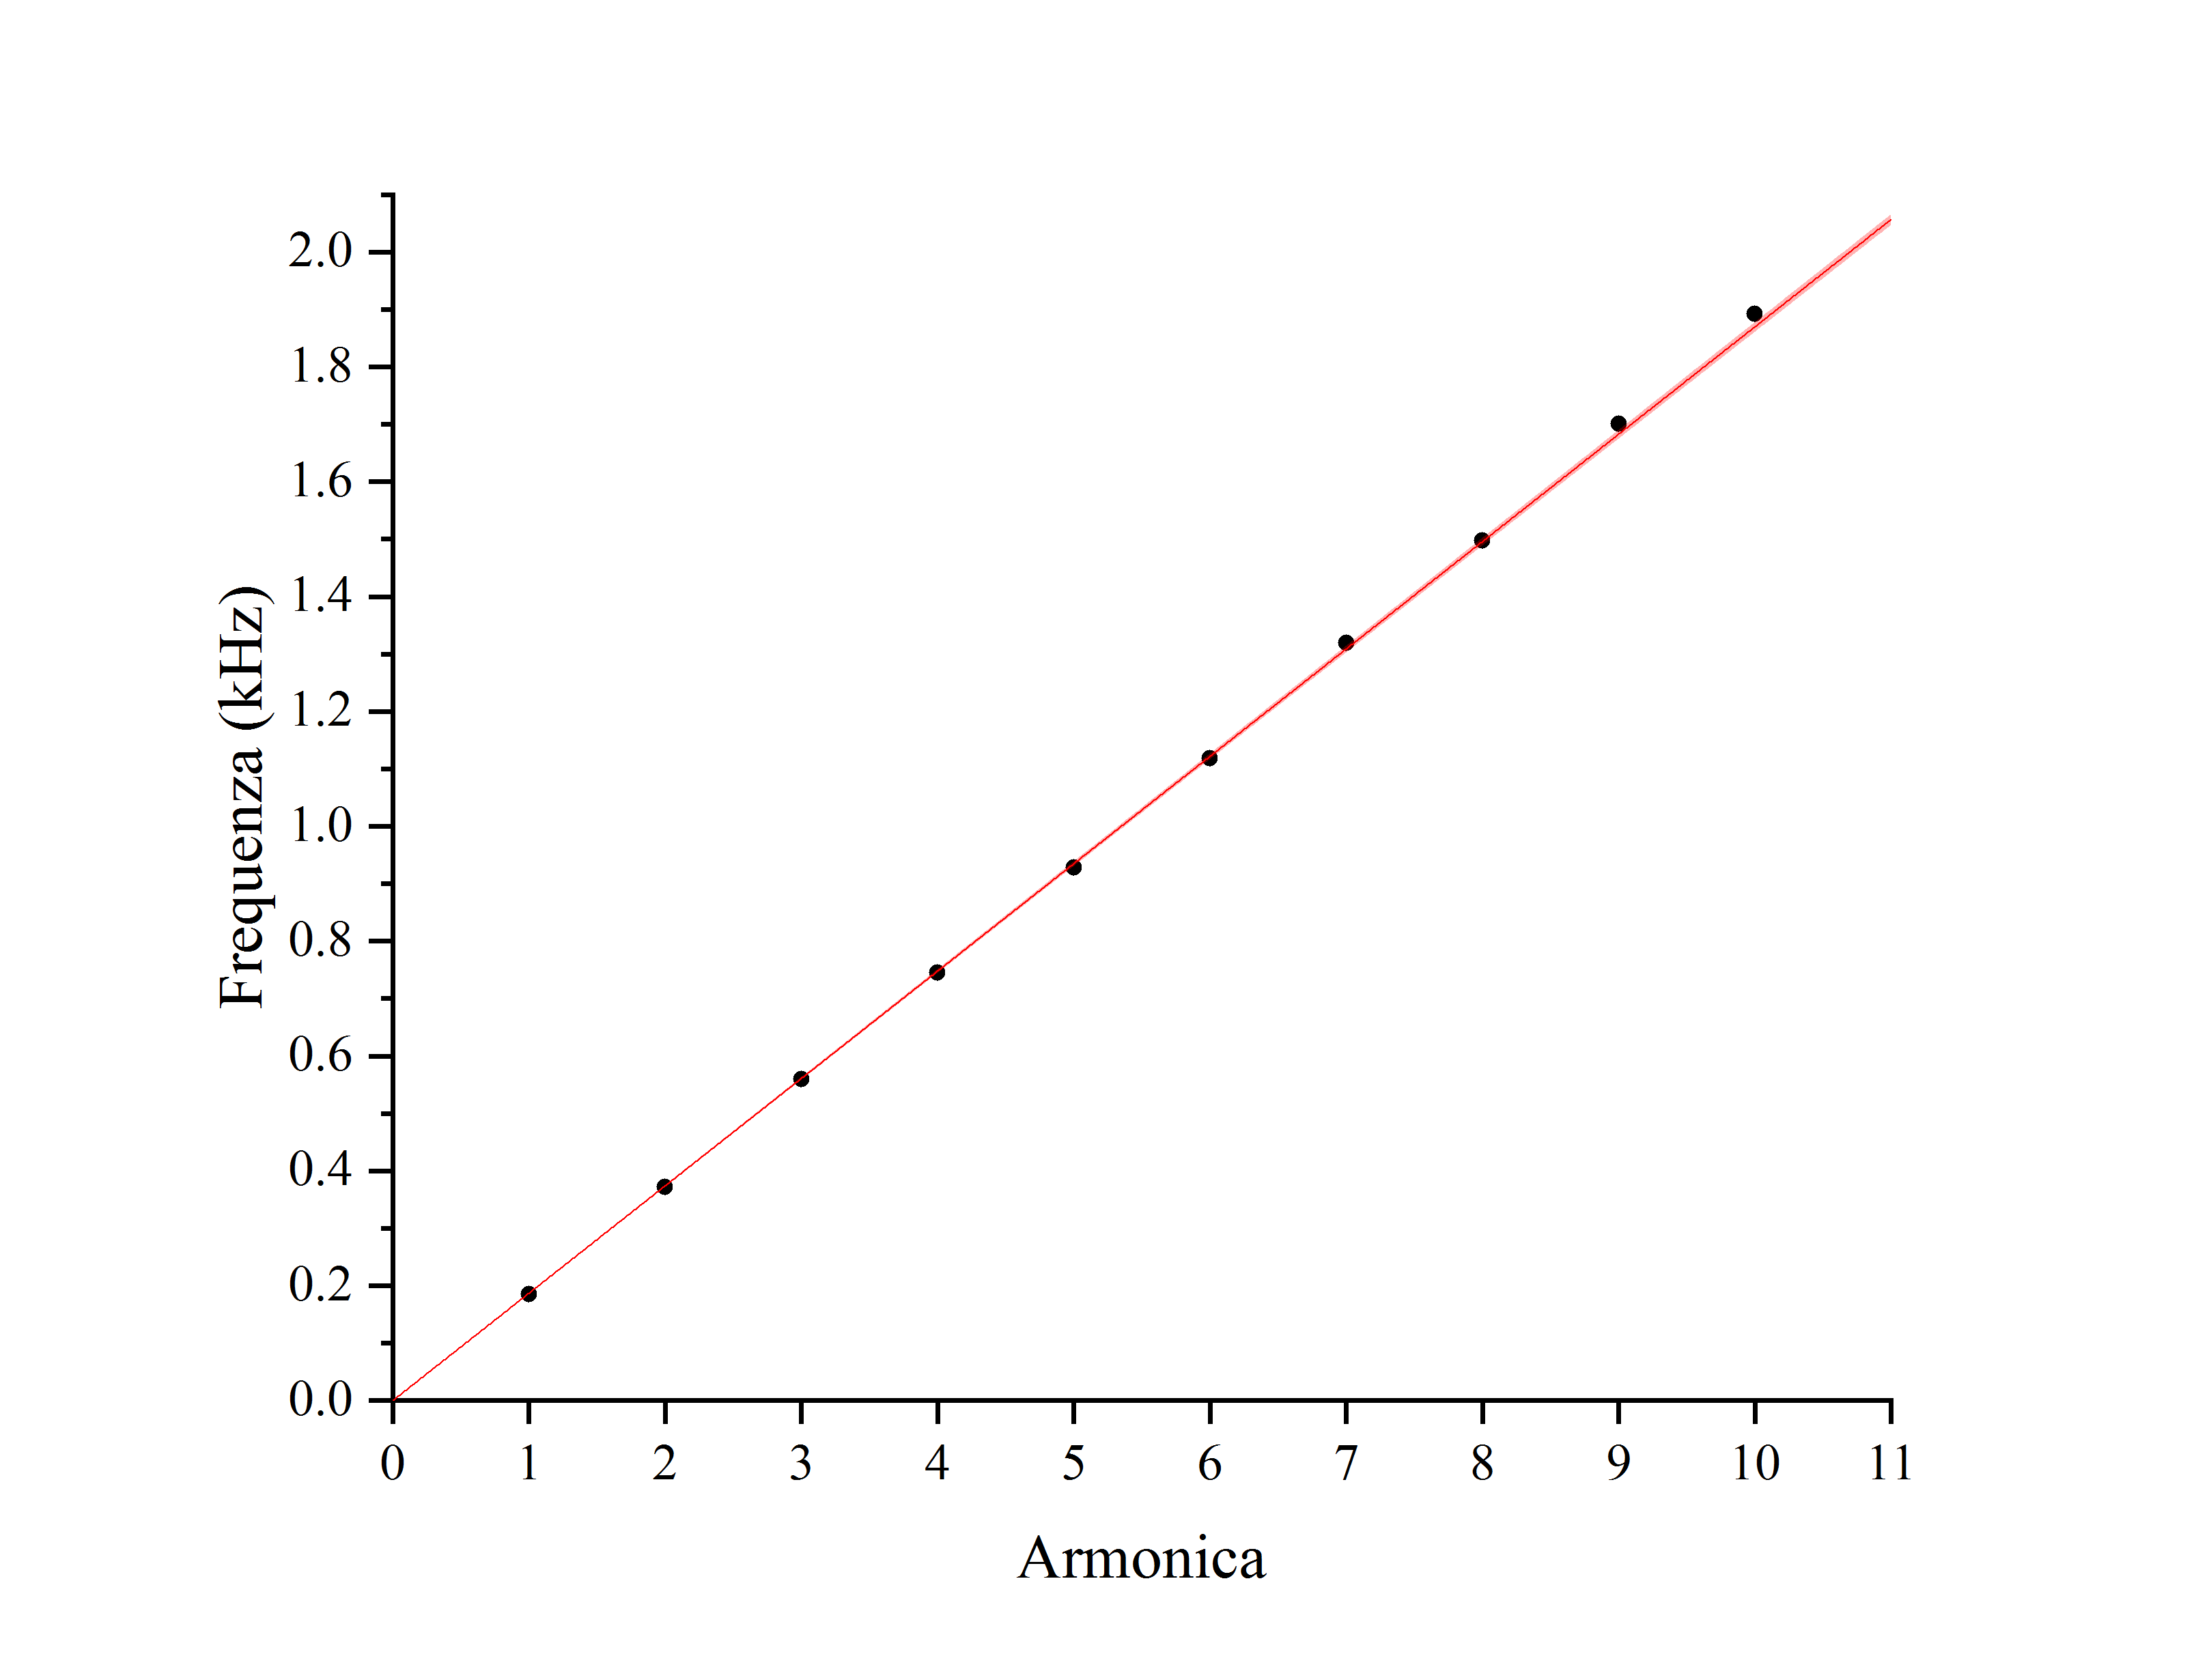
\includegraphics[trim={2.5cm 0.7cm 3cm 2cm},clip,width=0.47\textwidth]{img/l0r4.png}}\hfil
\end{figure}\begin{figure}[H]
  \centering
  \subfloat[][
    $L=(15.4\pm0.1)\;\unit{cm}$ \\
    $\xi^\text{c}=(509.5\pm0.1)\,\unit{Hz}$ \\
    $v=(345\pm2)\,\unit{m \per s}$
  ]{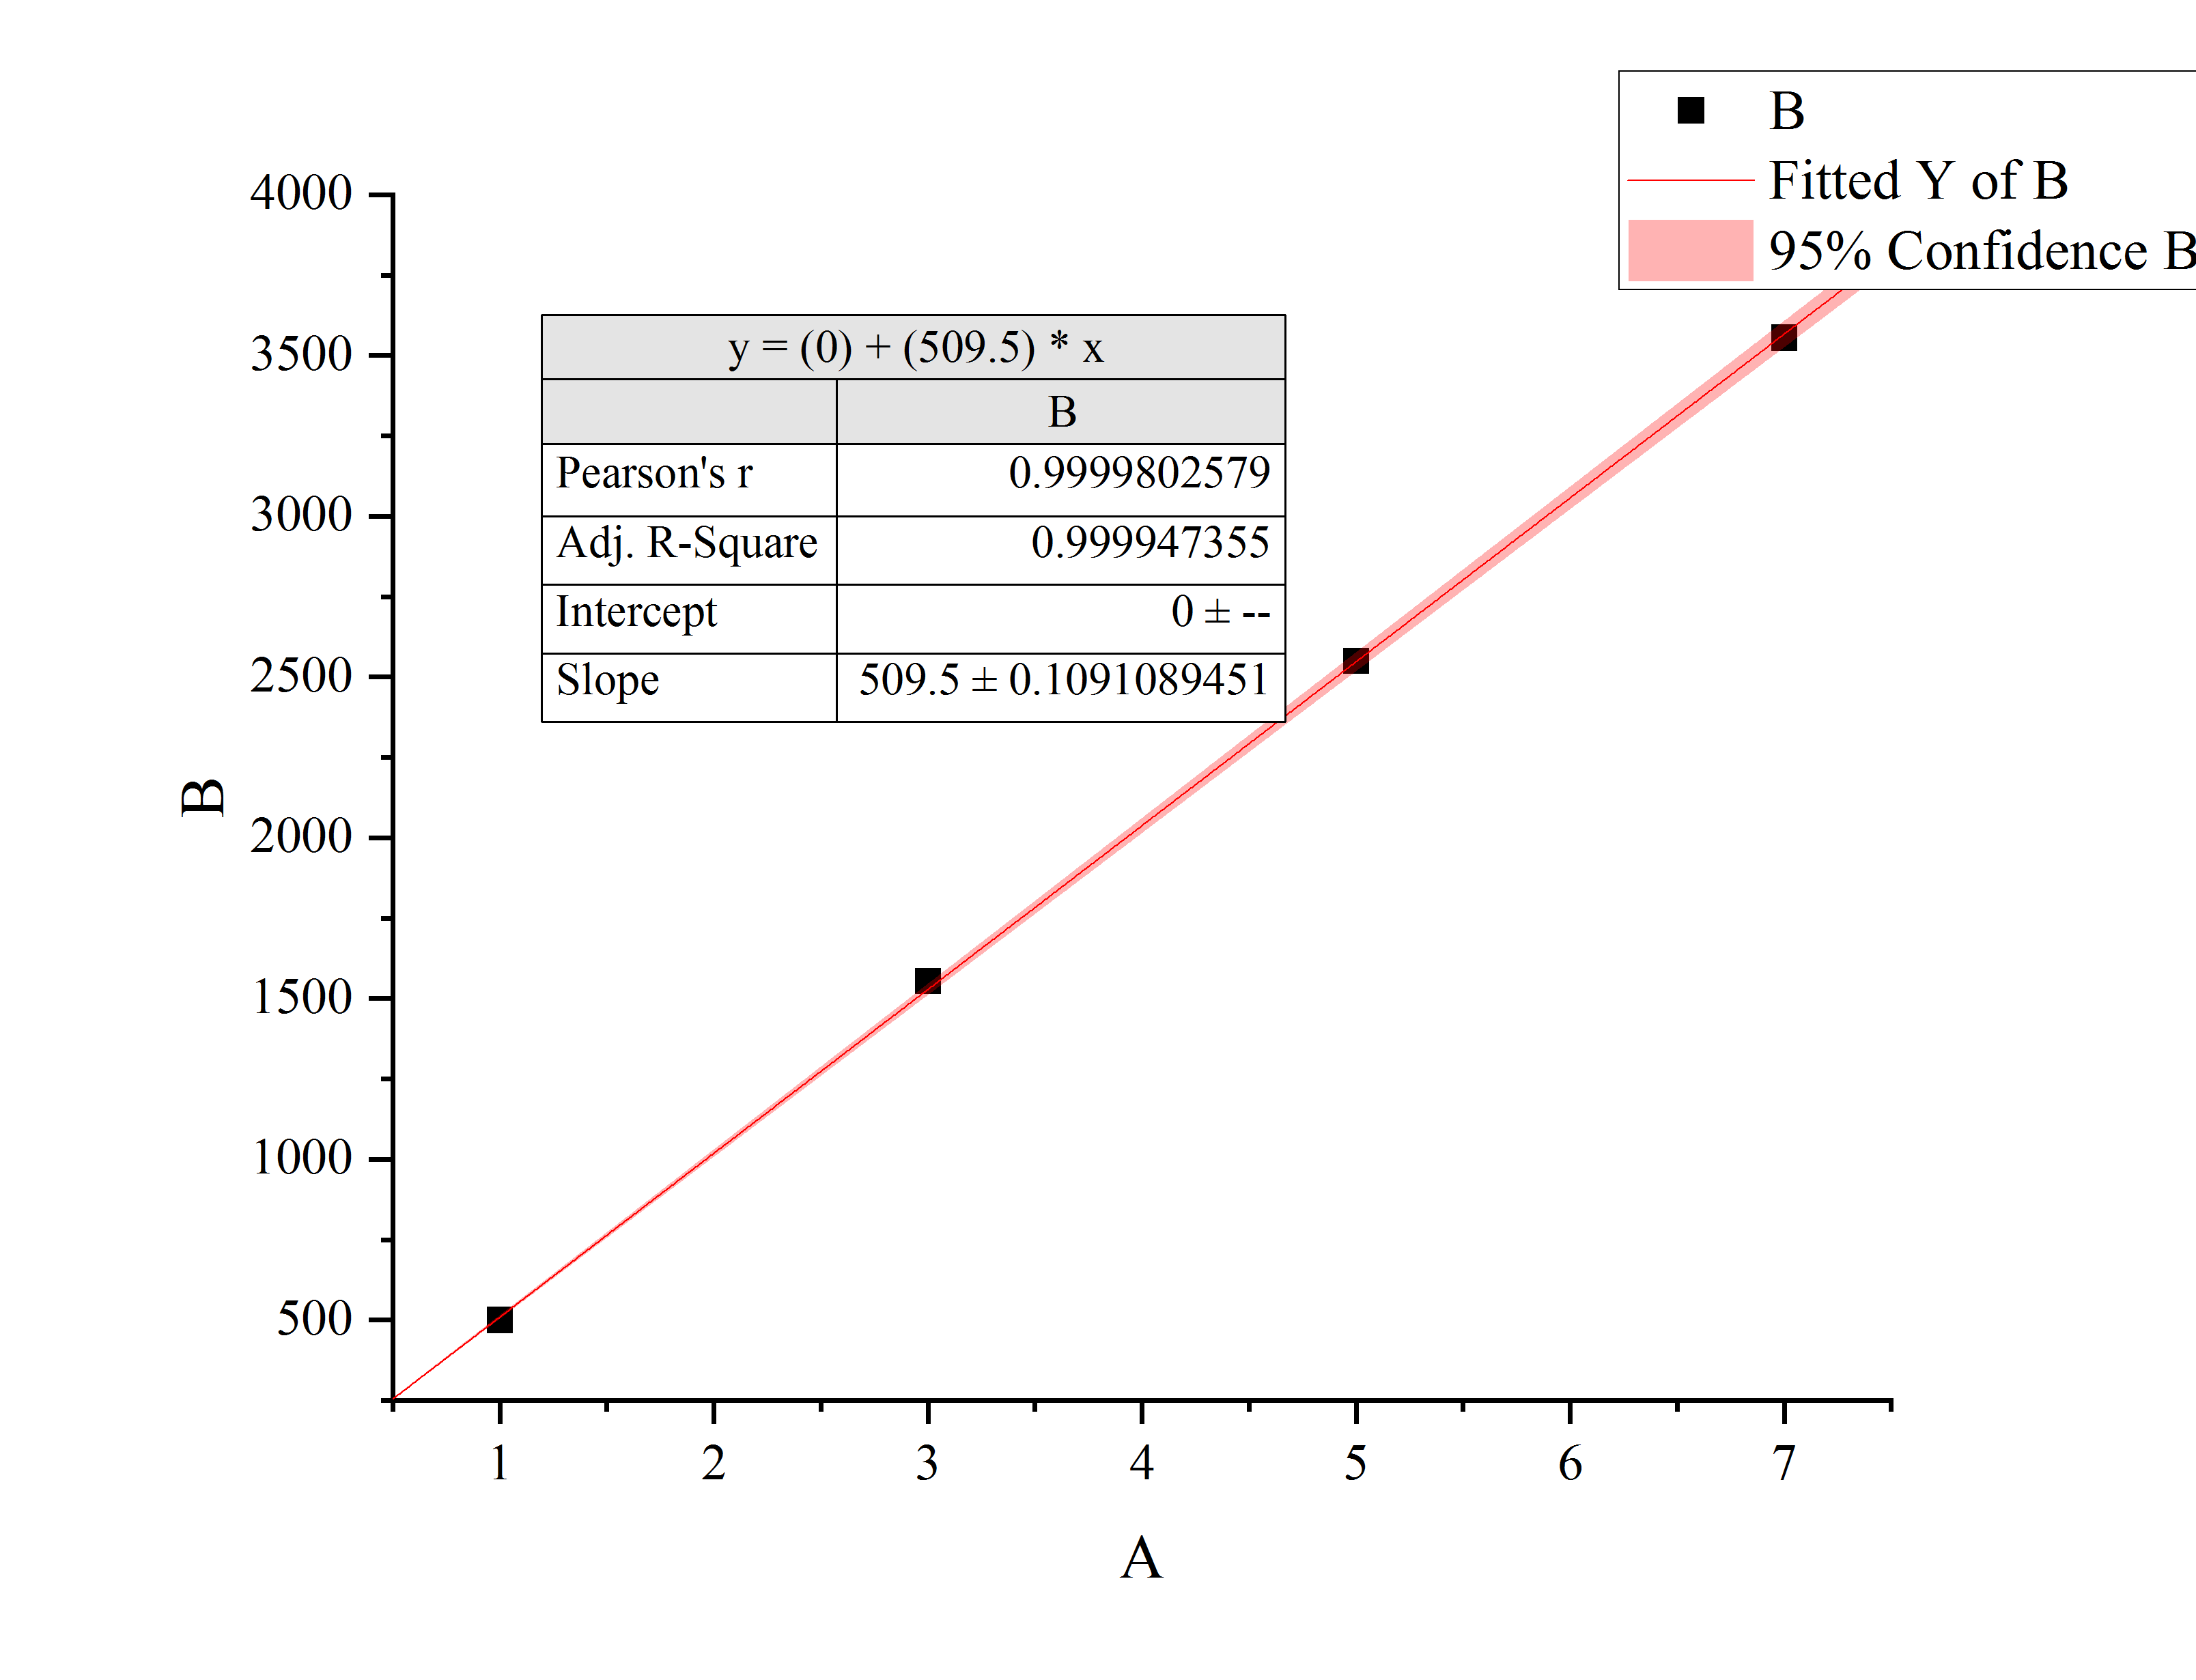
\includegraphics[trim={2.5cm 0.7cm 3cm 2cm},clip,width=0.47\textwidth]{img/l1.png}}\hfil
  \subfloat[][
    $L=(30.8\pm0.1)\;\unit{cm}$ \\
    $\xi^\text{c}=(267.00\pm0.06)\,\unit{Hz}$ \\
    $v=(345.3\pm1.1)\,\unit{m \per s}$
  ]{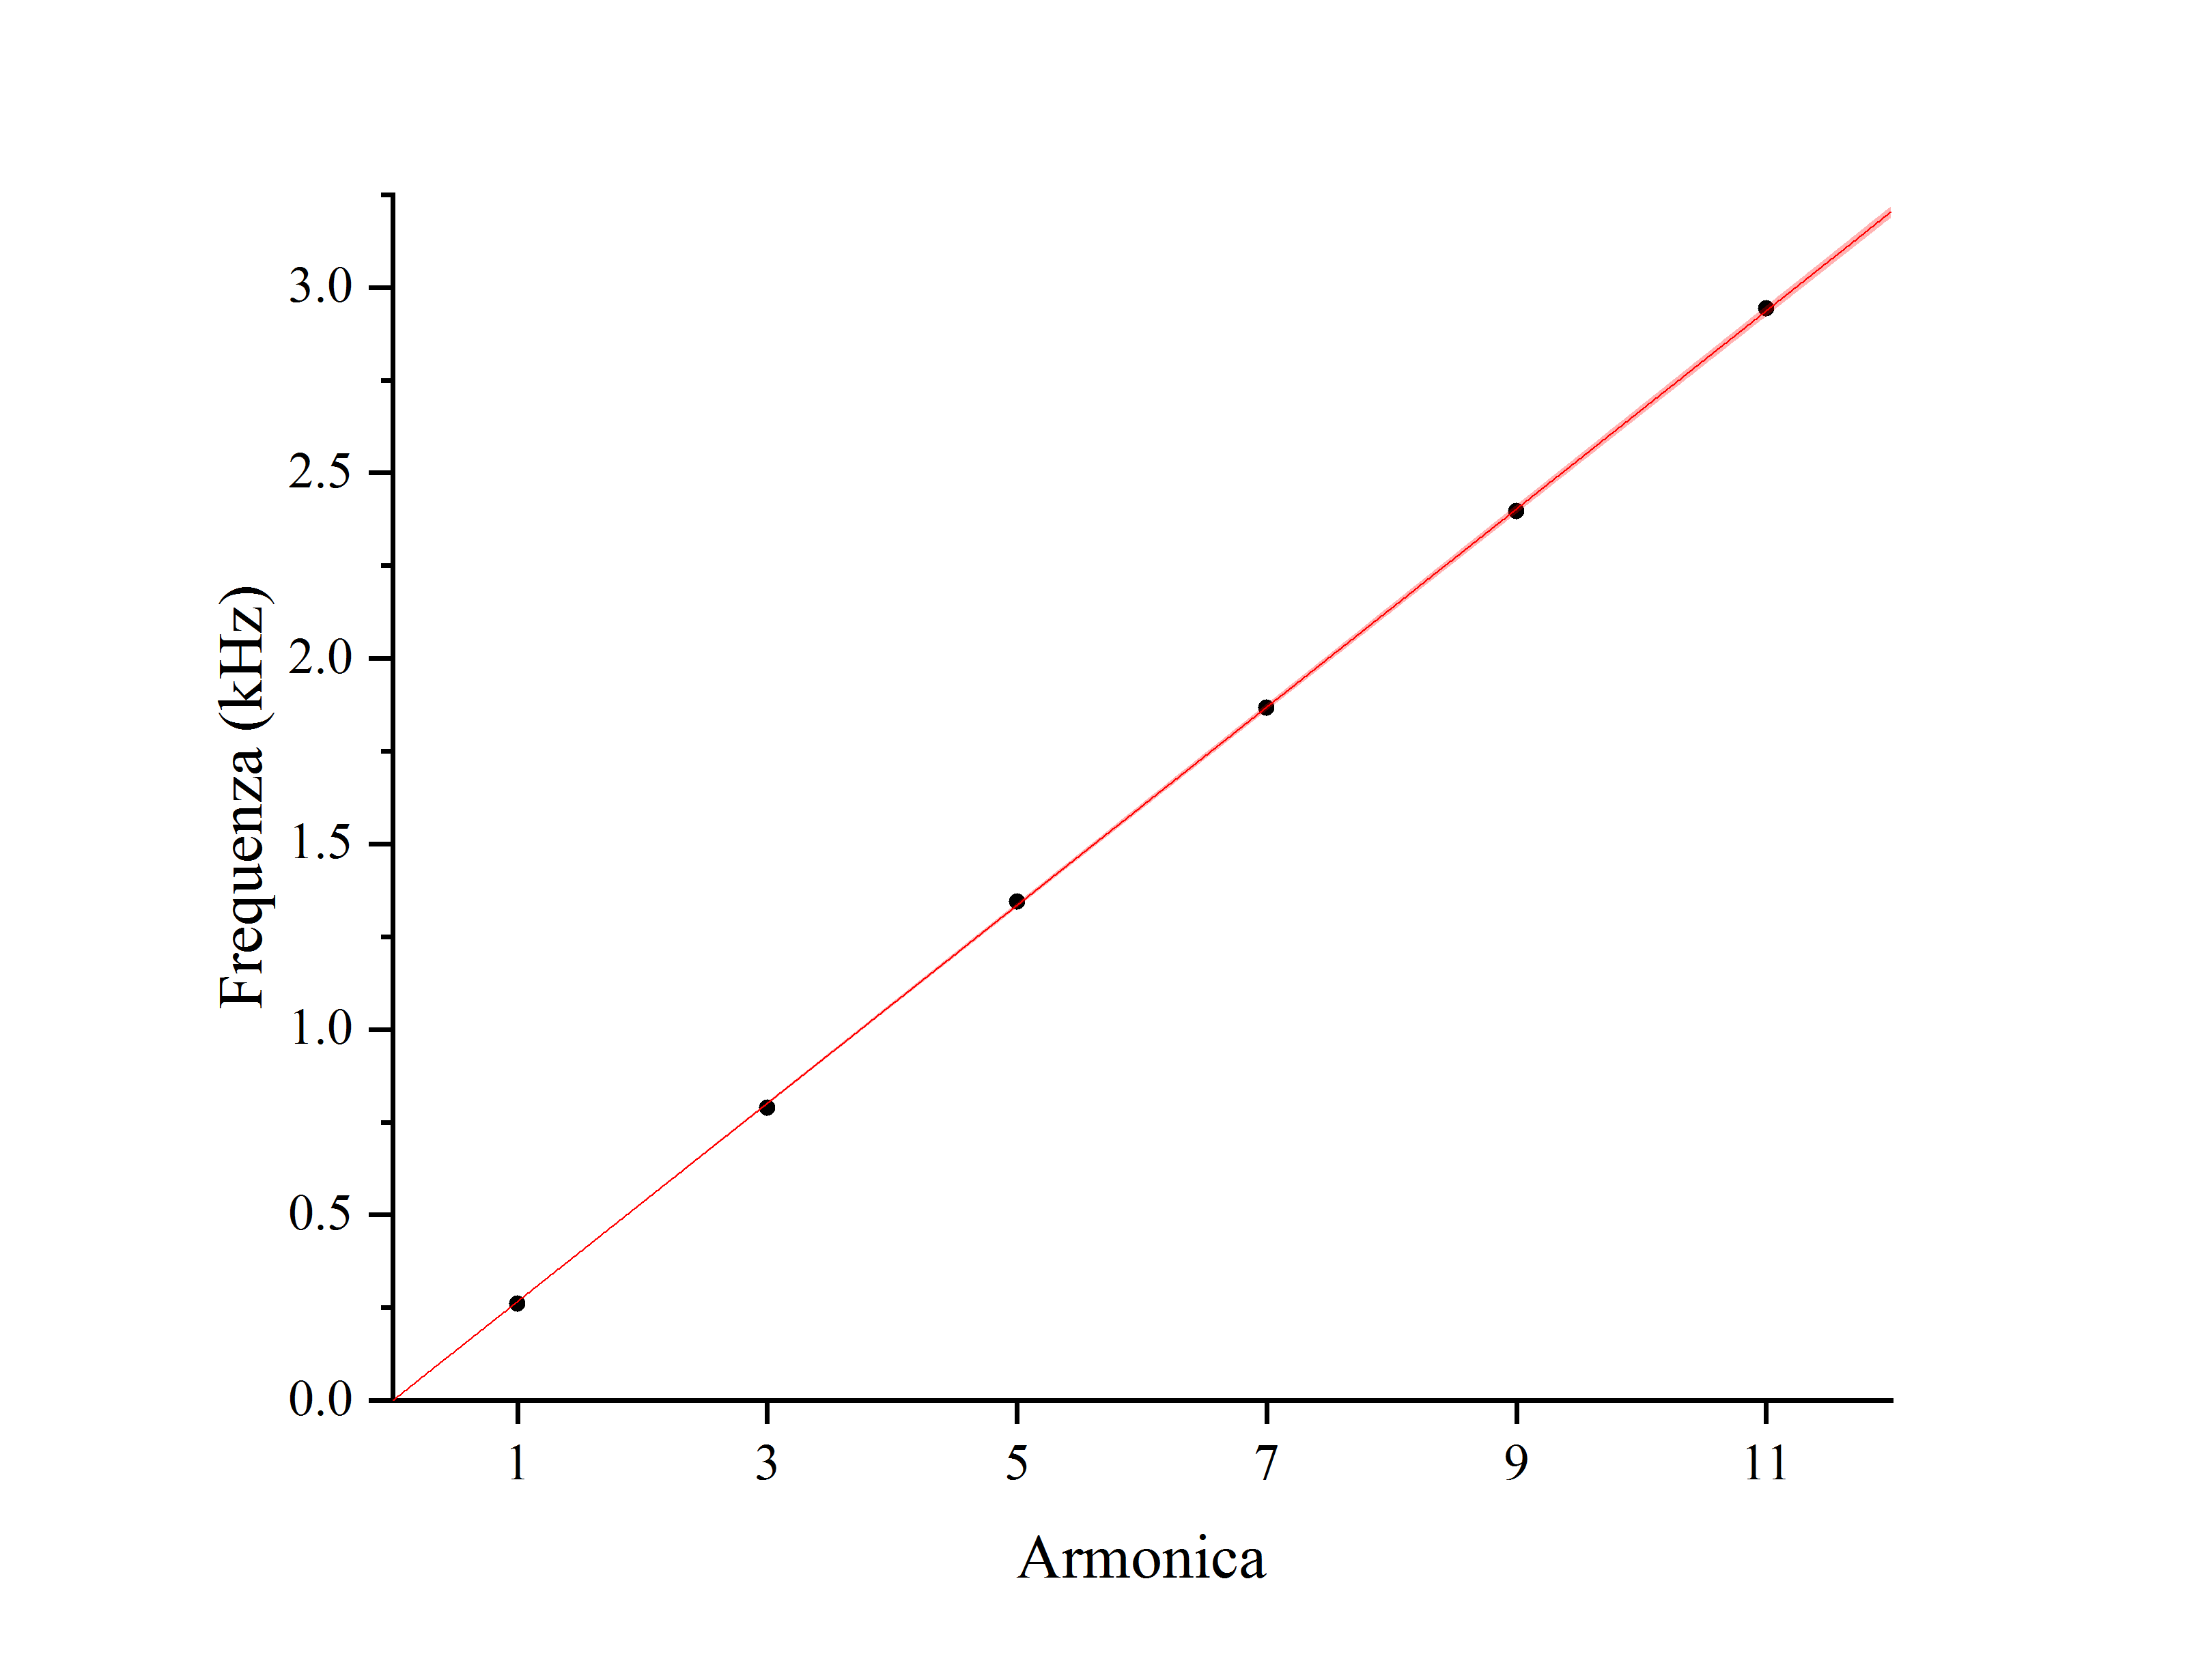
\includegraphics[trim={2.5cm 0.7cm 3cm 2cm},clip,width=0.47\textwidth]{img/l2.png}}\hfil
  \subfloat[][
    $L=(55.4\pm0.1)\;\unit{cm}$ \\
    $\xi^\text{c}=(152.12\pm0.06)\,\unit{Hz}$ \\
    $v=(346.4\pm0.7)\,\unit{m \per s}$
  ]{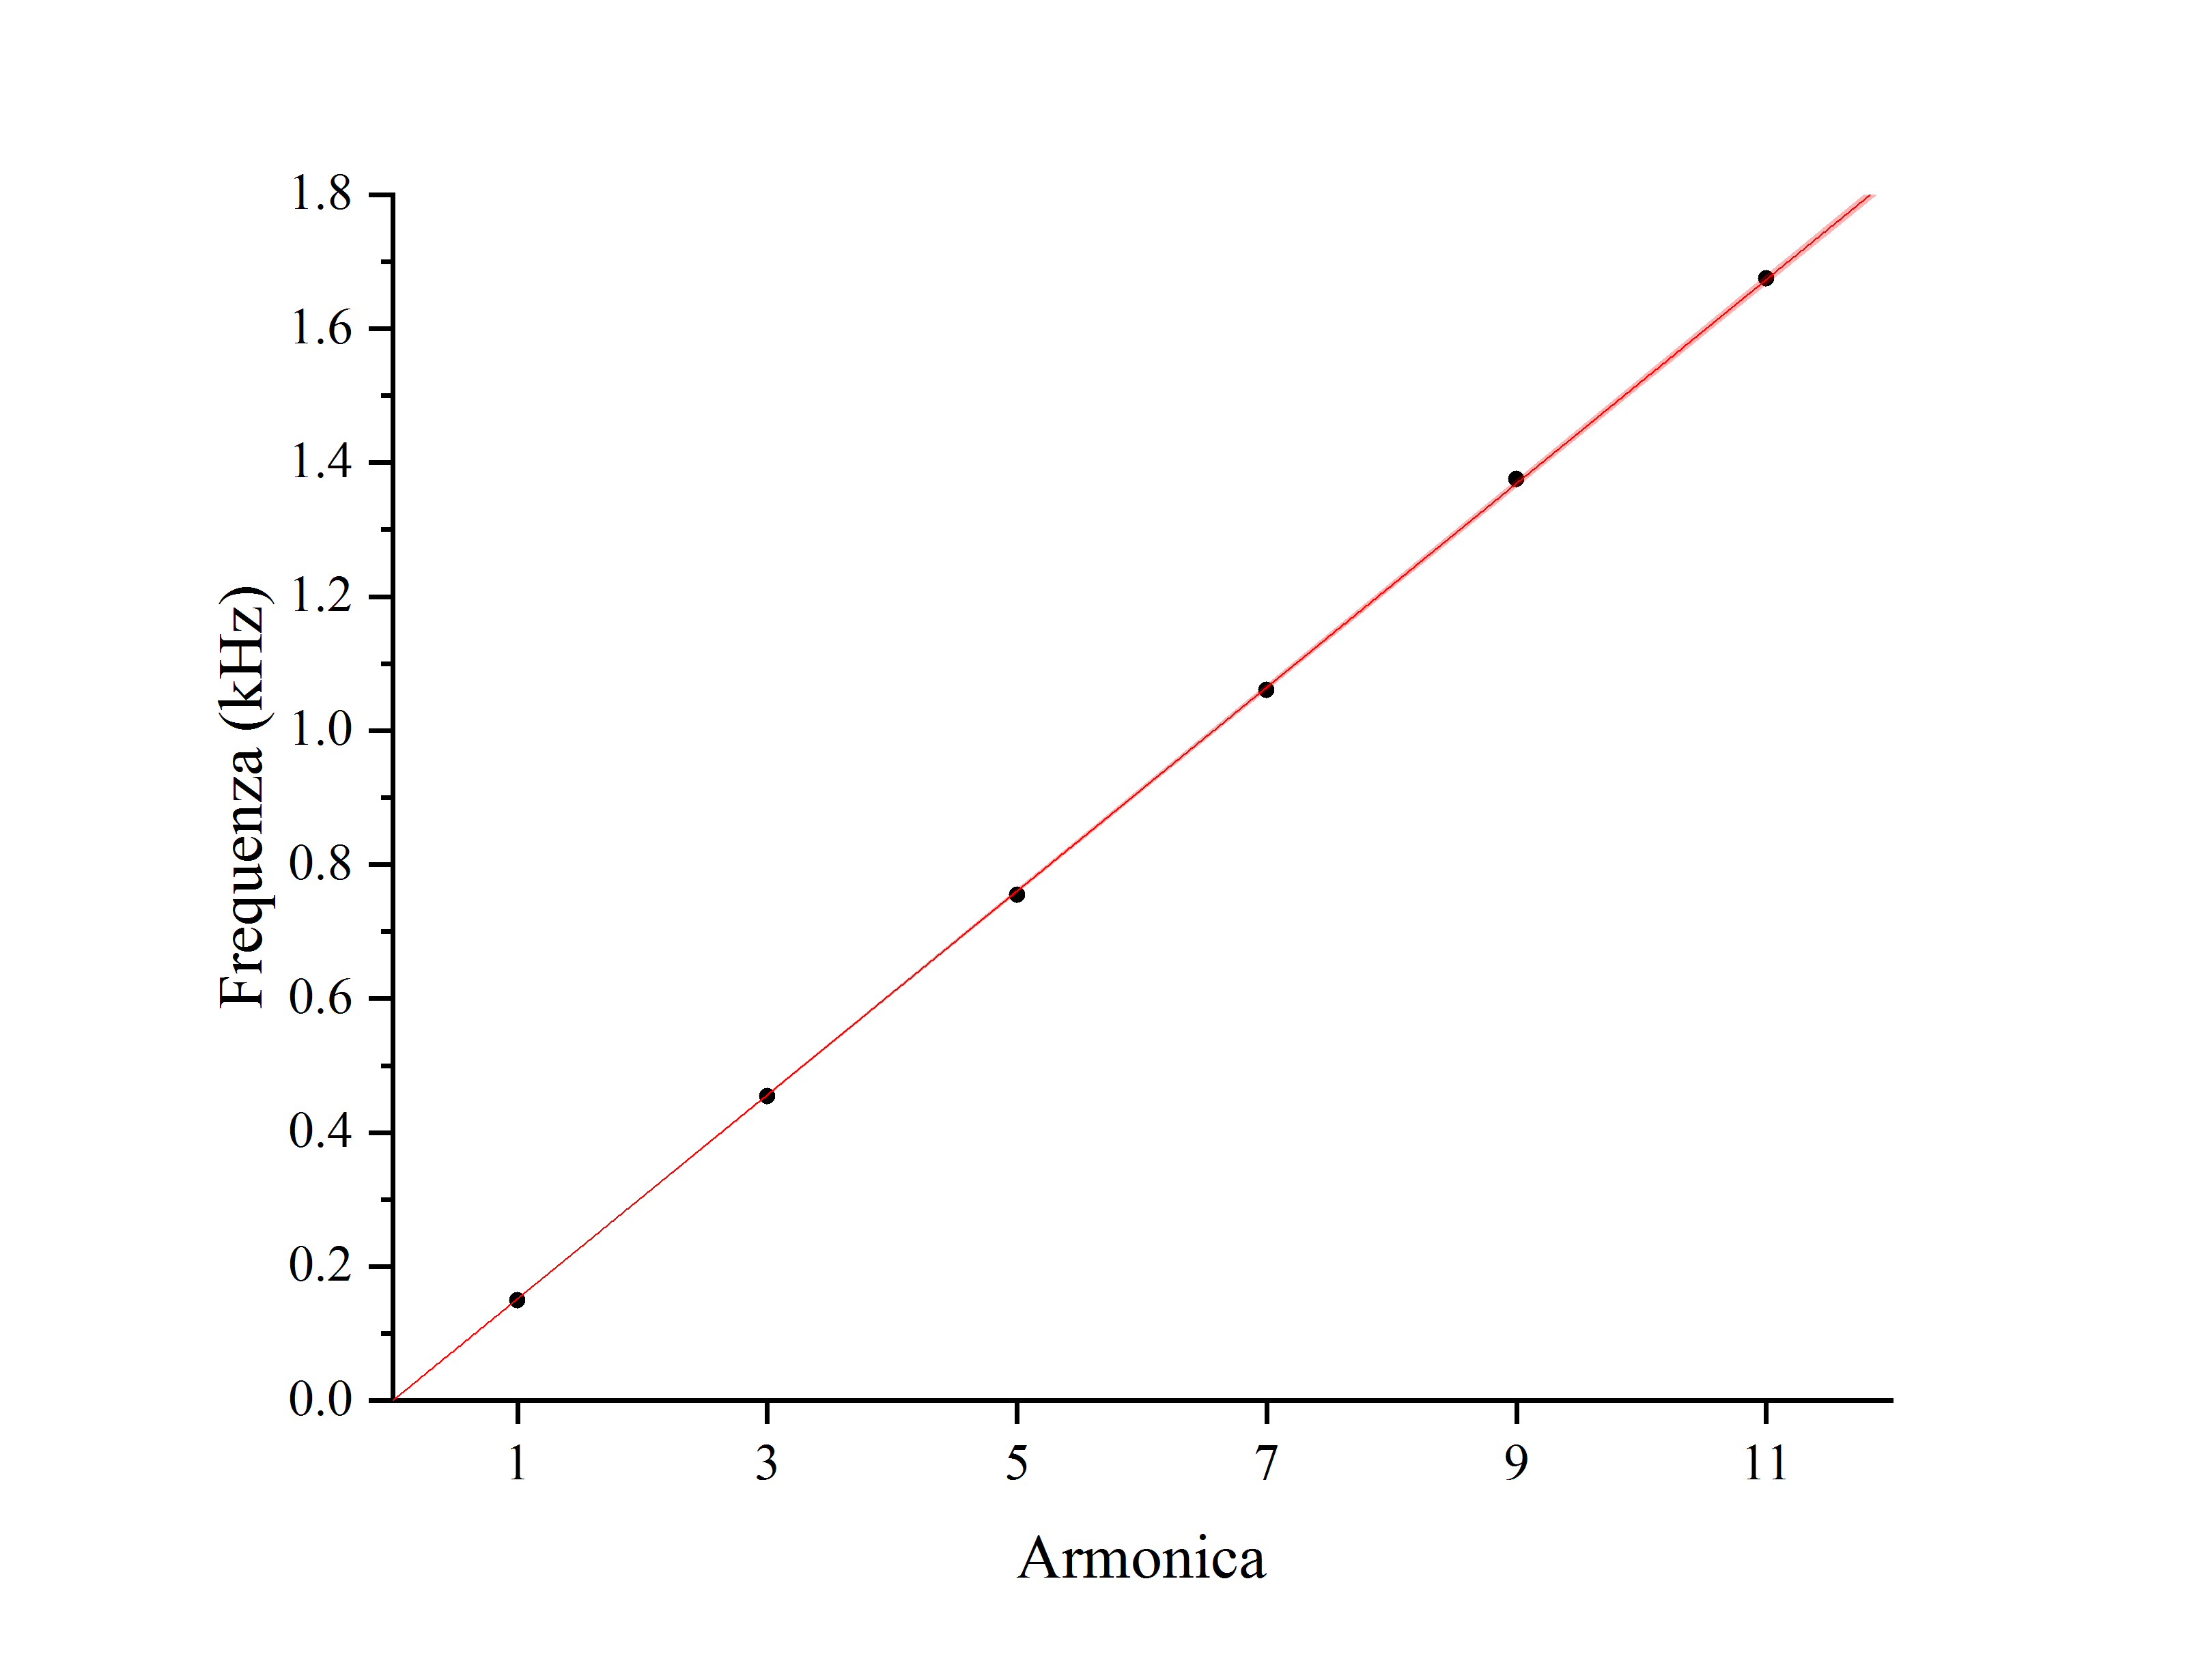
\includegraphics[trim={2.5cm 0.7cm 3cm 2cm},clip,width=0.47\textwidth]{img/l3.png}}\hfil
  \subfloat[][
    $L=(71.3\pm0.1)\;\unit{cm}$ \\
    $\xi^\text{c}=(118.64\pm0.06)\,\unit{Hz}$ \\
    $v=(345.6\pm0.6)\,\unit{m \per s}$
  ]{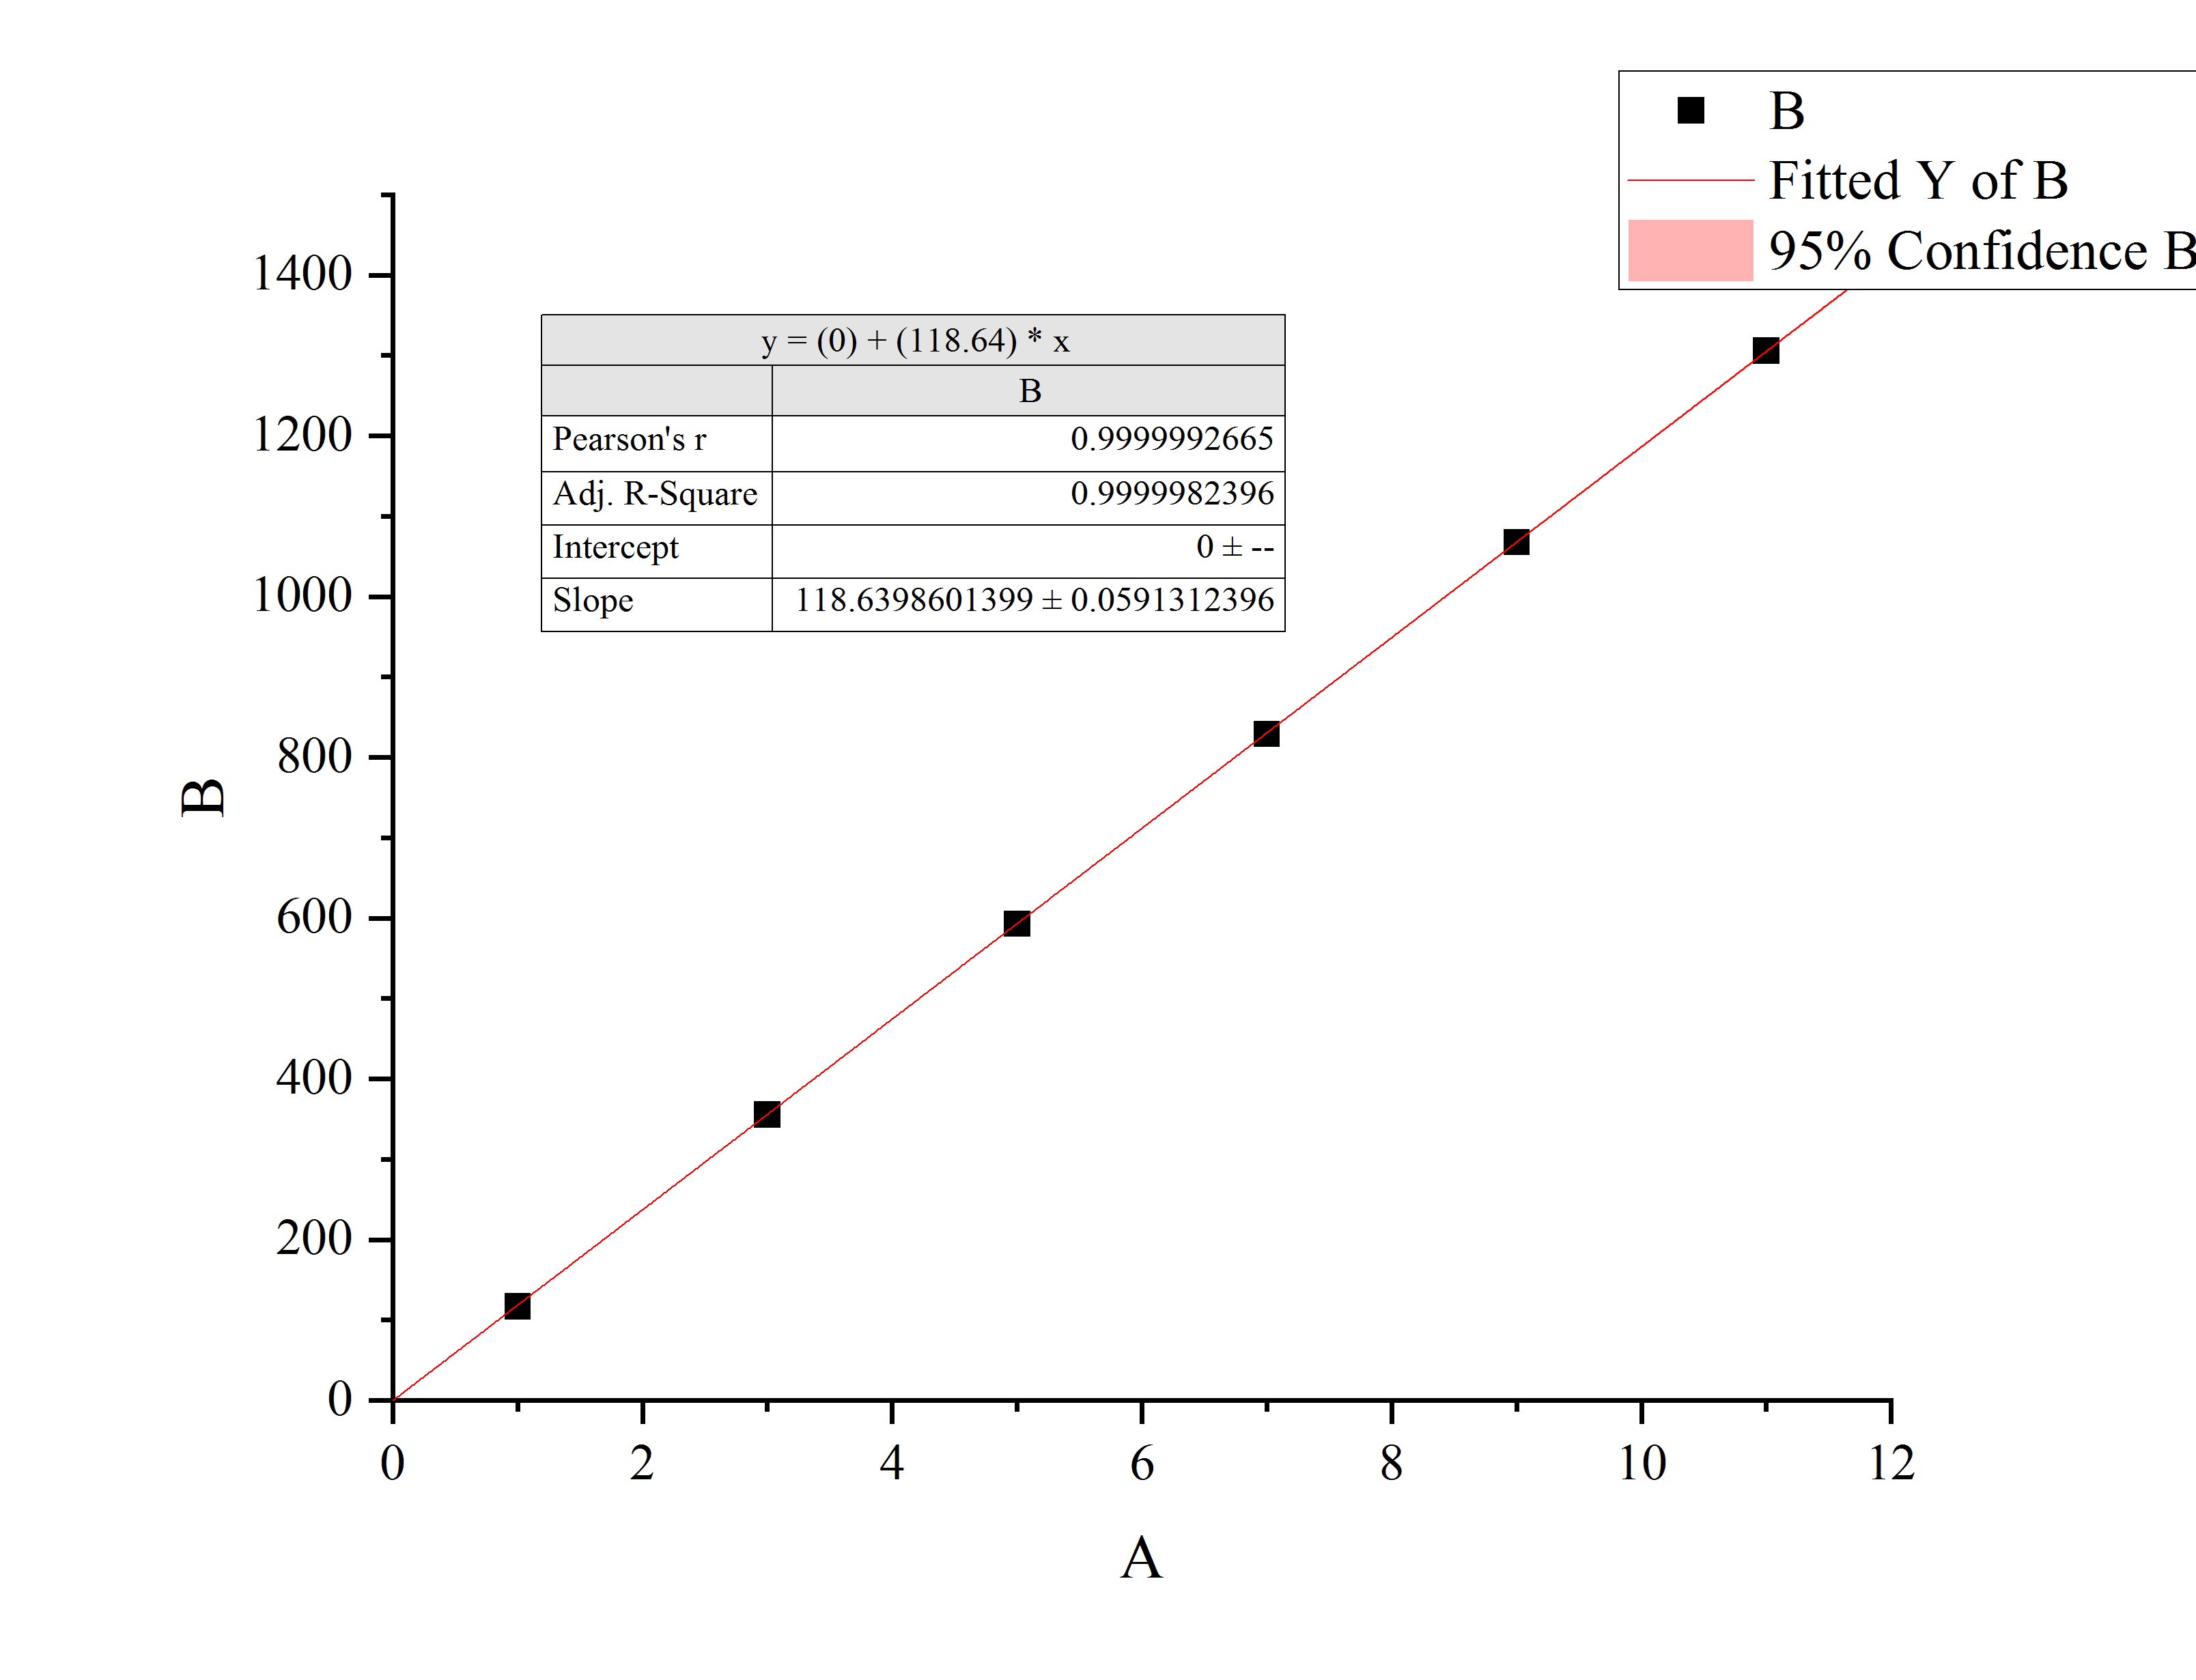
\includegraphics[trim={2.5cm 0.7cm 3cm 2cm},clip,width=0.47\textwidth]{img/l4.png}}\hfil
  \caption*{\emph{
    In rosso le rette di regressione e in rosa le rispettive regioni di incertezza.
    Le barre di errore, pur riportate, sono troppo ridotte per risultare visibili.
  }}
\end{figure}

\vspace{3mm}
\emph{
  \textbf{Osservazione.} È immediato notare, sulla base di questi grafici,
  che le rette di regressione, passanti per l'origine, descrivono accuratamente
  i dati raccolti: ciò suggerisce che la frequenza di risonanza più bassa da noi
  misurata sia effettivamente la fondamentale.
}

\subsection{Conclusioni}

Per valutare l'affidabilità delle misure di $v$ ottenute è
possibile confrontarle con la velocità del suono attesa
$v_\text{att}$, calcolata sulla base della temperatura
ambientale $T_\text{amb}$ durante l'esperienza, mediante una
relazione empirica:
\[
  v_\text{att}(T_\text{amb}) = (331.5 +
  \qty{0.607}{{\degree C}^{-1}}\,T_\text{amb})\,\unit{m \per s}
\]

Per quanto riguarda la prima misura, l'unica col tubo aperto,
la temperatura misurata era
$T_\text{amb}^\text{a} = (26.0\pm0.5)\,\unit{\degree C}$:
ne segue che $v_\text{att}^\text{a}=(347.3\pm0.3)\,\unit{m\per s}$.

Le altre misure, invece, sono state acquisite ad una
temperatura ambiente leggermente inferiore:
$T_\text{amb}^\text{c} = (24.5\pm0.5)\,\unit{\degree C}$,
da cui $v_\text{att}^\text{c} = (346.4\pm0.3)\,\unit{m\per s}$.

\vspace{2mm}
Come è possibile osservare comparando questi risultati a
quelli sopra riportati, tutti i valori di $v$ ottenuti
risultano compatibili con i rispettivi valori attesi.

\section{Misura mediante l'eco}

\subsection{Esperienza e procedimento di misura}

Ripetiamo quattro volte i seguenti passaggi:
\begin{enumerate}
  \item
    Mediante il termometro ambientale, misuriamo la temperatura ambiente
    $T_\text{amb}$ (in questo caso, abbiamo ottenuto, per tutte le misure,
    $T_\text{amb}=(25.5\pm0.5)\,\unit{\degree C}$).
  \item
    Chiusa l'estremità del tubo opposta all'altoparlante tramite il pistone,
    misuriamo la lunghezza $L$ della colonna d'aria all'interno del tubo.
  \item
    Accesi l'oscilloscopio e il generatore di onde, impostiamo una
    forma d'onda quadra e una frequenza di $(10\pm1)\,\unit{Hz}$.
    Regoliamo poi l'ampiezza fino a percepire un suono.
  \item
    Fissiamo il microfono appena sotto all'altoparlante, rivolto verso
    l'interno del tubo.
  \item
    Misuriamo, grazie all'oscilloscopio, un intervallo di tempo $\delta t$
    immediatamente successivo all'emissione dell'onda,
    in modo tale che i segnali delle eco siano chiaramente distinguibili.
    Contiamo allora, in quell'intervallo di tempo, il numero di picchi
    $N$ rilevati.
\end{enumerate}

\subsection{Analisi dei dati raccolti}

Sia $L_0$ la distanza percorsa dall'onda e sia $\Delta t_0$ il tempo
impiegato. Allora, chiaramente,
\[
  L_0 = 2L,
  \qquad
  \Delta t_0 = \frac{\Delta t}{N}
  \quad\text{e}\quad
  v = \frac{L_0}{\Delta t_0}.
\]

È quindi possibile stimare $v$ come il reciproco del coefficiente
angolare $\psi$ di una retta di regressione:
\[
  \Delta t_0 = \psi L_0
  \qquad\text{per cui}\quad v = \frac{1}{\psi}
\]

Di seguito riportiamo i valori di $L_0$ e $\Delta t_0$ da noi ottenuti,
accompagnati dai risultati della regressione lineare (pesata).

\begin{figure}[H]
  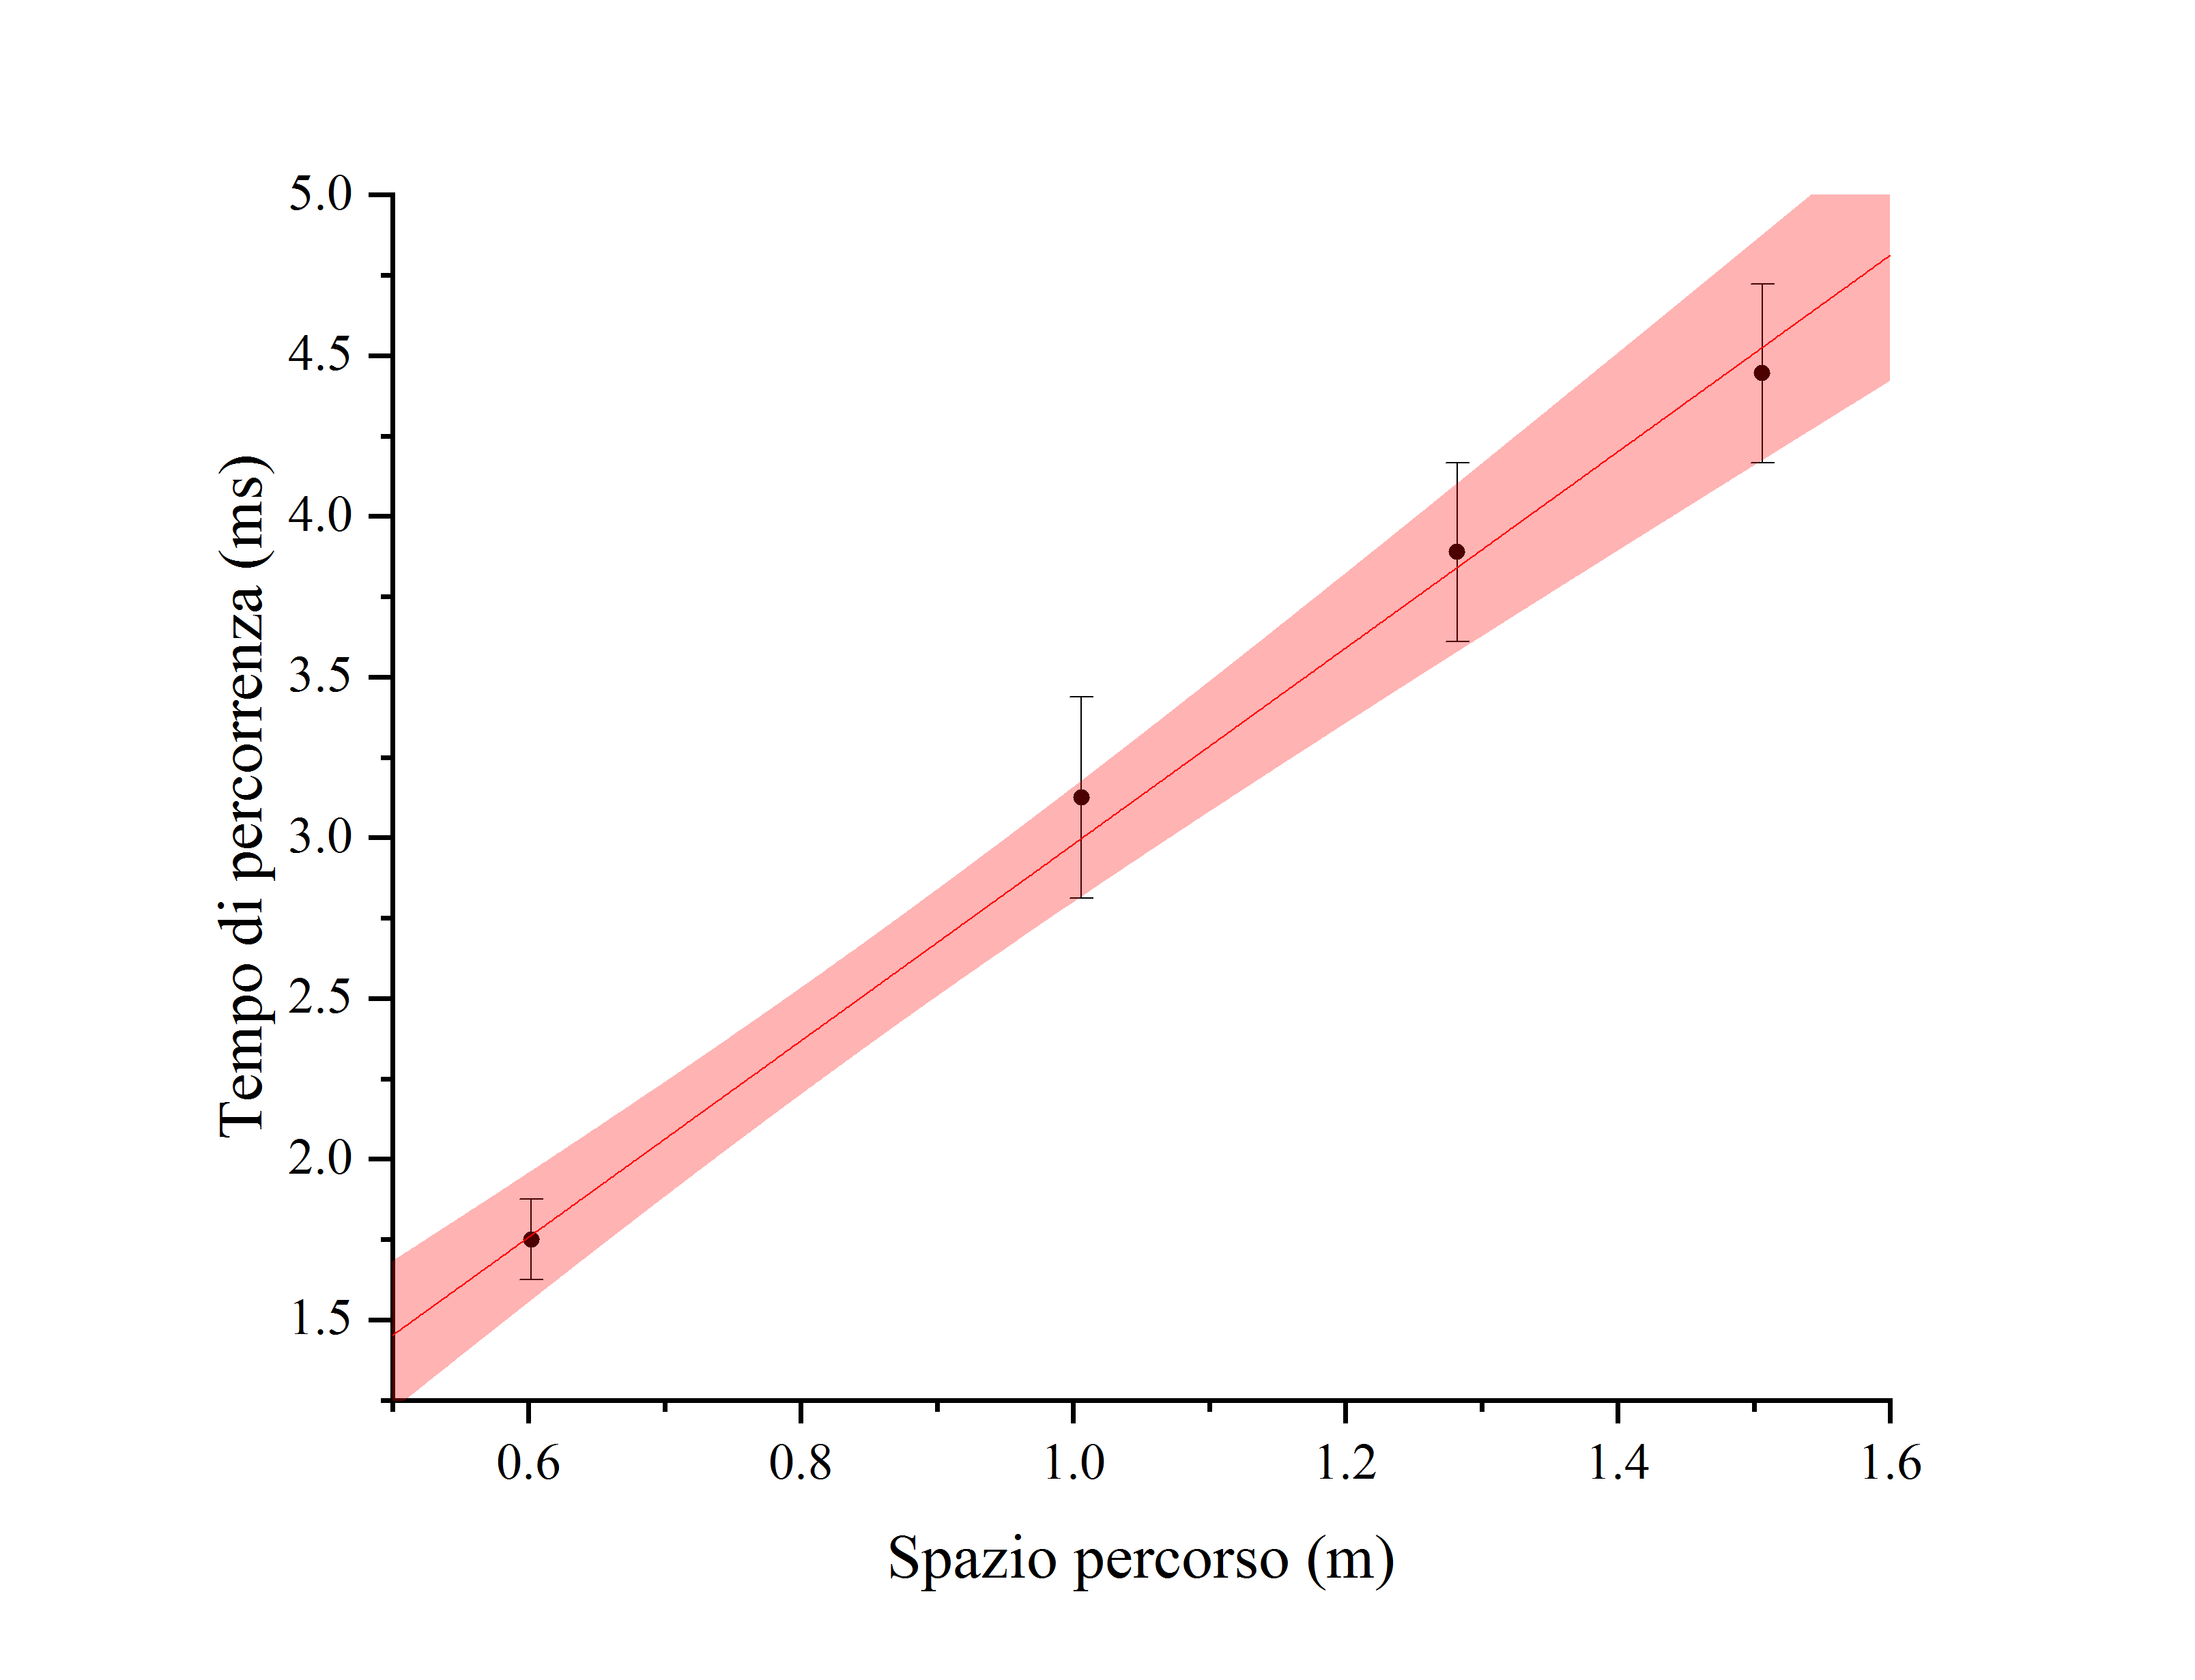
\includegraphics[trim={2.5cm 0.7cm 3cm 2cm},clip,width=\textwidth]{img/Graph2.png}
  \caption*{\emph{
    In rosso la retta di regressione, in rosa la sua regione di incertezza.
    Le barre di errore sull'ascissa, per quanto riportate nel grafico, non
    sono di dimensioni apprezzabili.
  }}
\end{figure}

\begin{itemize}
  \item Intercetta $= (-0.75 \pm 2.63)\cdot 10^{-4}\,\unit{s}$
  \item Coefficiente angolare $\psi = (3.05\pm0.29)\cdot 10^{-3}\,\unit{s\per m}$
\end{itemize}
da cui:
\[ v = (327 \pm 31)\,\unit{m \per s} \]

\pagebreak
\subsection{Conclusioni}
\emph{
  \textbf{Osservazione.}
  L'intercetta di questa retta di regressione è
  risultata compatibile con $0$, come ci si aspettava
  dalla relazione $\delta t_0 = \psi L_0$.
}

\vspace{2mm}
Per valutare l'affidabilità della stima di $v$ misurata,
possiamo confrontarla con un valore atteso $v_\text{att}$,
calcolato sulla base di $T_\text{amb}$ come mostrato nella
sezione precedente.

In questo caso, $v_\text{att} = (347.0\pm0.3)\,\unit{m \per s}$:
possiamo quindi affermare che la velocità del suono misurata
è abbondantemente compatibile con il valore atteso.

\vspace{5mm}
Possiamo pertanto concludere che l'esperienza ha avuto successo:
mediante l'apparato sperimentale il gruppo di lavoro ha ottenuto
misure della velocità del suono compatibili con quelle attese.

\end{document}
